El objetivo del trabajo es dise'nar e implementar un protocolo para el reparto de cartas y juego de Truco Mental entre dos jugadores.
El protocolo est'a dise'nado para garantizar una justa repartici'on de cartas y que cada parte juege s'olo cartas que le fueron repartidas.

El lenguaje elegido es Python, y la implementaci'on realizada permite que dos jugadores juegen una mano a trav'es de una conexi'on por red. Al ejecutar el programa, 'este pregunta si debe ser ejecutado en modo cliente o modo servidor. Si se ejecutaran varias instancias del servidor en la misma computadora, se podr'ia dar un servicio de truco a varios jugadores simult'anea e independientemente.

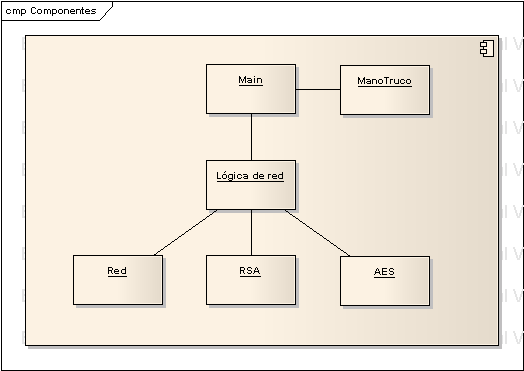
\includegraphics{Componentes.png}